% Options for packages loaded elsewhere
\PassOptionsToPackage{unicode}{hyperref}
\PassOptionsToPackage{hyphens}{url}
%
\documentclass[
]{article}
\usepackage{lmodern}
\usepackage{amsmath}
\usepackage{ifxetex,ifluatex}
\ifnum 0\ifxetex 1\fi\ifluatex 1\fi=0 % if pdftex
  \usepackage[T1]{fontenc}
  \usepackage[utf8]{inputenc}
  \usepackage{textcomp} % provide euro and other symbols
  \usepackage{amssymb}
\else % if luatex or xetex
  \usepackage{unicode-math}
  \defaultfontfeatures{Scale=MatchLowercase}
  \defaultfontfeatures[\rmfamily]{Ligatures=TeX,Scale=1}
\fi
% Use upquote if available, for straight quotes in verbatim environments
\IfFileExists{upquote.sty}{\usepackage{upquote}}{}
\IfFileExists{microtype.sty}{% use microtype if available
  \usepackage[]{microtype}
  \UseMicrotypeSet[protrusion]{basicmath} % disable protrusion for tt fonts
}{}
\makeatletter
\@ifundefined{KOMAClassName}{% if non-KOMA class
  \IfFileExists{parskip.sty}{%
    \usepackage{parskip}
  }{% else
    \setlength{\parindent}{0pt}
    \setlength{\parskip}{6pt plus 2pt minus 1pt}}
}{% if KOMA class
  \KOMAoptions{parskip=half}}
\makeatother
\usepackage{xcolor}
\IfFileExists{xurl.sty}{\usepackage{xurl}}{} % add URL line breaks if available
\IfFileExists{bookmark.sty}{\usepackage{bookmark}}{\usepackage{hyperref}}
\hypersetup{
  pdftitle={ASCOT ADAPT Trial Simulation Report},
  hidelinks,
  pdfcreator={LaTeX via pandoc}}
\urlstyle{same} % disable monospaced font for URLs
\usepackage[margin=1in]{geometry}
\usepackage{longtable,booktabs}
\usepackage{calc} % for calculating minipage widths
% Correct order of tables after \paragraph or \subparagraph
\usepackage{etoolbox}
\makeatletter
\patchcmd\longtable{\par}{\if@noskipsec\mbox{}\fi\par}{}{}
\makeatother
% Allow footnotes in longtable head/foot
\IfFileExists{footnotehyper.sty}{\usepackage{footnotehyper}}{\usepackage{footnote}}
\makesavenoteenv{longtable}
\usepackage{graphicx}
\makeatletter
\def\maxwidth{\ifdim\Gin@nat@width>\linewidth\linewidth\else\Gin@nat@width\fi}
\def\maxheight{\ifdim\Gin@nat@height>\textheight\textheight\else\Gin@nat@height\fi}
\makeatother
% Scale images if necessary, so that they will not overflow the page
% margins by default, and it is still possible to overwrite the defaults
% using explicit options in \includegraphics[width, height, ...]{}
\setkeys{Gin}{width=\maxwidth,height=\maxheight,keepaspectratio}
% Set default figure placement to htbp
\makeatletter
\def\fps@figure{htbp}
\makeatother
\setlength{\emergencystretch}{3em} % prevent overfull lines
\providecommand{\tightlist}{%
  \setlength{\itemsep}{0pt}\setlength{\parskip}{0pt}}
\setcounter{secnumdepth}{5}
\usepackage{booktabs}
\usepackage{blkarray}
\usepackage{pdflscape}
\usepackage{lastpage}
\usepackage{vhistory}
\usepackage{titling}
\usepackage{fontspec}
\pretitle{\begin{center}

\includegraphics[width=2in,height=2in]{../image.jpg}\LARGE\\}
\posttitle{\end{center}}
\newcommand{\blandscape}{\begin{landscape}}
\newcommand{\elandscape}{\end{landscape}}
\usepackage{fancyhdr}
\pagestyle{fancy}
\fancyhf{}
\fancyhead[LO]{ASCOT ADAPT Statistical Appendix}
\fancyfoot[LO]{Version 2.0, October, 2020}
\fancyfoot[RO]{\thepage\ of \pageref{LastPage}}
\renewcommand{\headrulewidth}{0pt}
\renewcommand{\footrulewidth}{0pt}
\setlength{\headheight}{14pt}

\setromanfont[Ligatures=TeX]{Latin Modern Roman}
\setsansfont[Ligatures=TeX]{Latin Modern Sans}
\setmonofont[Ligatures=TeX]{Latin Modern Mono}
\setmathfont[Ligatures=TeX]{Latin Modern Math}
\renewcommand{\familydefault}{\sfdefault}
\usepackage{booktabs}
\usepackage{longtable}
\usepackage{array}
\usepackage{multirow}
\usepackage{wrapfig}
\usepackage{float}
\usepackage{colortbl}
\usepackage{pdflscape}
\usepackage{tabu}
\usepackage{threeparttable}
\usepackage{threeparttablex}
\usepackage[normalem]{ulem}
\usepackage{makecell}
\usepackage{xcolor}
\ifluatex
  \usepackage{selnolig}  % disable illegal ligatures
\fi

\title{ASCOT ADAPT Trial Simulation Report}
\usepackage{etoolbox}
\makeatletter
\providecommand{\subtitle}[1]{% add subtitle to \maketitle
  \apptocmd{\@title}{\par {\large #1 \par}}{}{}
}
\makeatother
\subtitle{Version 1.1}
\author{}
\date{\vspace{-2.5em}January 2021}

\begin{document}
\maketitle

{
\setcounter{tocdepth}{2}
\tableofcontents
}
\hypertarget{version-history}{%
\section*{Version History}\label{version-history}}
\addcontentsline{toc}{section}{Version History}

\begin{center}
    \begin{tabular}{lllp{5cm}}
    \hline
    Version & Date & Author & Description \\ \hline
    1.0 & August 2020  & JT & Initial simulation results \\ 
    1.1 & January 2021 & JT & Change to RAR scheme where minimum allocation of 1/3 enforced. \\ 
    \hline
    \end{tabular}
\end{center}

\clearpage

\hypertarget{introduction}{%
\section{Introduction}\label{introduction}}

This document is a supplement to the ASCOT ADAPT trial core protocol.
It outlines the technical details of the clinical trial simulations and results used in planning the ASCOT ADAPT trial decision thresholds.
The simulations are used to understand the operating characteristics of the platform trial under various design configurations.
This is a living document where trial scenarios or trial summaries may be added as required.
For full details of the analysis plan refer to the Statistical Analysis Appendix.

\clearpage

\hypertarget{simulation-design}{%
\section{Simulation Design}\label{simulation-design}}

\hypertarget{model}{%
\subsection{Model}\label{model}}

The primary endpoint in the trial is death from any cause or requirement of new intensive respiratory support (invasive or non-invasive ventilation) or vasopressor/inotropic support in the 28 days after randomisation.
This endpoint is binary and in these simulations a participants response is coded as 1 if they died or required new intensive respiratory support or vasopressor/inotropic support ventilation-free to 28 days and is 0 if they did not.
Therefore, a beneficial treatment is one which reduces the probability of response.
The outcome is modelled by logistic regression and treatment effects are expressed in terms of their reduction in the log-odds of the outcome.

\hypertarget{domains}{%
\subsubsection{Domains}\label{domains}}

For the purposes of this simulation document, 3 domains have been considered.
To make the document generalisable, these domains and the comprising treatments are not explicitly denoted, but are treated as generic.

The generic domains considered are labelled:

\begin{itemize}
\tightlist
\item
  Domain \(A\), consisting of 4 treatment combinations \(A_0.A_1,A_2,A_3\). Treatment \(A_0\) is the absence of any treatment from domain \(A\) (standard of care).
\item
  Domain \(B\), consisting of 3 treatments \(B_0,B_1,B_2\). Treatment \(B_0\) is the absence of any domain \(B\) treatment.
\item
  Domain \(C\), consisting of 2 treatments \(C_0,C_1\).
\end{itemize}

A regimen is a combination of one treatment option from each domain.
Every participant receives one regimen.
The number of unique regimens in these simulations, assuming all combinations are viable, is \(4\times 3\times 2=24\).

The model used in these simulations are, for a given participant \(i\)
\[
\begin{aligned}
\eta_i &= \beta_0 + x_{A(i)}^{\mathsf{T}}\beta_A + x_{B(i)}^{\mathsf{T}}\beta_B + x_{C(i)}^{\mathsf{T}}\beta_C \\
\pi_i &= \text{logit}^{-1}(\eta_i)
\end{aligned}, \quad i=1,2,3,...
\]
where \(\eta_i\) is there participants linear predictor as given by the combination of treatments they receive and \(\pi_i\) is the participants probability of ventilation-free survival by 28 days after enrolment.

The vectors, e.g.~\(x_{A(i)}\), select the relevant parameters from \(\beta_A\), for example if participant \(i\) receives treatment \(A_5\) then \(x_{A(i)}^{\mathsf{T}} = (0\ 1\ 1\ 0\ 0\ 1)\) where \(\beta_{A1}\) is the effect of treatment \(A_1\) alone, \(\beta_{A2}\) is the effect of \(A_2\) alone, and \(\beta_{A5}\) is the interaction effect between \(A_1\) and \(A_2\) when given in combination.
This complete set of treatment option within a domain is expressed by the design matrix.
For example, domain \(A\) has design
\[
 X_{A} = 
\begin{blockarray}{ccccccc}
          & \beta_{A0} & \beta_{A1} & \beta_{A2} & \beta_{A3} \\
\begin{block}{r(cccccc)}
      A_0 & 1 & 0 & 0 & 0 \\
      A_1 & 0 & 1 & 0 & 0 \\
      A_2 & 0 & 0 & 1 & 0 \\
      A_3 & 0 & 0 & 0 & 1 \\
\end{block}
\end{blockarray}
\]
and the notation \(A(i)\) indicates which row of the design matrix \(X_A\) applies for participant \(i\).

The current model does not allow for interactions between separate domains, all treatment effects within domains are therefore assumed to be additive in combination.

\hypertarget{prior}{%
\subsubsection{Prior}\label{prior}}

The prior distributions for the parameters are
\[
\begin{aligned}
\beta_0 &\sim N(0, 10^2) \\
\beta_{A0},\beta_{B0},\beta_{C0} &= 0 \\
\beta_{A1},\beta_{A2},\beta_{A3},\beta_{B1},\beta_{B2},\beta_{C1} &\sim N(0, 1).
\end{aligned}
\]
For identifiability, the effect of receiving \(A_0\),\(B_0\) and \(C_0\) are set to zero implying that \(\beta_0\) is the log-odds of response when no treatments are received in any domain (standard of care).

\hypertarget{model-quantities}{%
\subsubsection{Model Quantities}\label{model-quantities}}

For the purpose of decision making, expected response under each regimen is of primary interest.
Define
\[
\begin{aligned}
\eta_j &= \beta_0 + x_{A(j)}^{\mathsf{T}}\beta_A + x_{B(j)}^{\mathsf{T}}\beta_B + x_{C(j)}^{\mathsf{T}}\beta_C \\
\pi_j &= \text{logit}^{-1}(\eta_j)
\end{aligned},\quad j=1,...,48
\]
to be the log-odds and probability of response under regimen \(j\).
As before, the notation \(A(j)\in\{0,1,2,3\}\) indicates which combination of domain \(A\) treatments forms regimen \(j\).

The parameters of primary interest are the treatment effects relative to no treatment (or another treatment within the domain) and the best treatment within each domain.

In what follows, all probabilities are implicitly conditional on the model and available data at the time of the analysis.

\textbf{Best Regimen}

Define \(j^\star = \text{argmin}_j \eta_j\) to be the regimen which minimises the log-odds of response.
The probability that regimen \(j\) is the best regimen (in terms of minimising the log-odds of response) is
\[
\mathbb P[\text{regimen }j\text{ is best}] = \mathbb P[j^\star = j] = \mathbb P[\eta_j < \eta_{l}, l\ne j],\quad j=1,...,48.
\]

\textbf{Best Treatment}

Define the probability that a treatment combination within each domain \(A\), \(B\), and \(C\) is in the best regimen by
\[
\begin{aligned}
\mathbb P[\text{treatment }A_k\text{ is in best}] = \mathbb P[A(j^\star)=k],&\quad k=0,1,2,3 \\
\mathbb P[\text{treatment }B_k\text{ is in best}] = \mathbb P[B(j^\star)=k],&\quad k=0,1,2 \\
\mathbb P[\text{treatment }C_k\text{ is in best}] = \mathbb P[C(j^\star)=k],&\quad k=0,1
\end{aligned}.
\]

\textbf{Treatment Comparisons}

Define the probability that a treatment combination has a lower log-odds of the outcome than another treatment combination by
\[
\begin{aligned}
\mathbb P[\text{treatment }A_k\text{ better than treatment } A_l] &=\mathbb P\left[x_{A(k)}^{\mathsf{T}}\beta_A < x_{A(l)}^{\mathsf{T}}\beta_A\right],\quad k,l\in\{0,1,2,3\} \\
\mathbb P[\text{treatment }B_k\text{ better than treatment } B_l] &=\mathbb P\left[x_{B(k)}^{\mathsf{T}}\beta_B < x_{B(l)}^{\mathsf{T}}\beta_B\right],\quad k,l\in\{0,1,2\} \\
\mathbb P[\text{treatment }C_k\text{ better than treatment } C_l] &=\mathbb P\left[x_{C(k)}^{\mathsf{T}}\beta_C < x_{C(l)}^{\mathsf{T}}\beta_C\right],\quad k,l\in\{0,1\}
\end{aligned}
\]

For example, the probability that treatment \(A_2\) reduces the log-odds of response compared to \(A_0\) is
\[
\mathbb P[\text{treatment } A_5\text{ better than treatment } A_0] = \mathbb P[\beta_{A2}<0].
\]

\hypertarget{decisions-and-adaptations}{%
\subsection{Decisions and Adaptations}\label{decisions-and-adaptations}}

A variety of trial decisions and adaptations may be possible as the trial progresses, for example, dropping the no treatment option within a domain if at least one treatment is found effective (reduces the log-odds of response compared to no treatment), or dropping all other treatment options if one treatment is found superior to all others (results in the lowest log-odds of response amongst all treatments).

Example decisions and their definitions are provided in Table \ref{tab:dectab}.
These example decisions are presented for a single treatment, \(A_5\).
Not all decisions will be defined or of interest for all treatment combinations and these examples are indicative only.
Some of the treatments overlap and some definitions are redundant in that they can be defined in terms of other decisions (e.g.~harm is contained in futility and inferiority is the complement of superiority).

\begin{table}[H]

\caption{\label{tab:dectab}Example trial decisions and definitions.}
\centering
\begin{tabular}[t]{lllll}
\toprule
Decision & Comparison & Quantity & Threshold & Action\\
\midrule
$A_5$ is effective & $A_5$ vs $A_0$ & $\mathbb P[\beta_{A1}+\beta_{A2}+\beta_{A5}<0]$ & 0.99 & Drop $A_0$\\
$A_5$ is harmful & $A_5$ vs $A_0$ & $\mathbb P[\beta_{A1}+\beta_{A2}+\beta_{A5}>0]$ & 0.99 & Drop $A_5$\\
$A_5$ is futile & $A_5$ vs $A_0$ & $\mathbb P[\beta_{A1}+\beta_{A2}+\beta_{A5}>-\Delta]$ & 0.95 & Drop $A_5$\\
$A_5$ is equivalent & $A_5$ vs $A_0$ & $\mathbb P[|\beta_{A1}+\beta_{A2}+\beta_{A5}|<\Delta]$ & 0.90 & Drop $A_5$\\
$A_5$ is futile & $A_5$ vs $A_1$ & $\mathbb P[\beta_{A2}+\beta_{A5}>-\Delta]$ & 0.95 & Drop $A_5$\\
$A_5$ is futile & $A_5$ vs $A_2$ & $\mathbb P[\beta_{A1}+\beta_{A5}>-\Delta]$ & 0.95 & Drop $A_5$\\
$A_5$ is superior & $A_5$ vs all $A$ & $\mathbb P[A(j^\star)=5]$ & 0.99 & Drop all $A$ except $A_5$\\
$A_5$ is inferior & $A_5$ vs all $A$ & $\mathbb P[A(j^\star)\ne5]$ & 0.99 & Drop $A_5$\\
\bottomrule
\end{tabular}
\end{table}

For completeness, the actual decisions and thresholds used in the trial simulations for domain \(A\) are given in Table \ref{tab:simdectab}.
The decisions for domains \(B\) and \(C\) are similar except for the absence of the extra futility check for a combination treatment.

\begin{table}[H]

\caption{\label{tab:simdectab}Simulation trial decisions and thresholds $(\Delta = \ln(1.1))$}
\centering
\begin{tabular}[t]{lllll}
\toprule
Decision & Comparison & Quantity & Threshold & Action\\
\midrule
$A_1$ is effective & $A_1$ vs $A_0$ & $\mathbb P[\beta_{A1}<0]$ & $>0.99$ & Drop $A_0$\\
$A_2$ is effective & $A_2$ vs $A_0$ & $\mathbb P[\beta_{A2}<0]$ & $>0.99$ & Drop $A_0$\\
$A_3$ is effective & $A_3$ vs $A_0$ & $\mathbb P[\beta_{A3}<0]$ & $>0.99$ & Drop $A_0$\\
$A_4$ is effective & $A_4$ vs $A_0$ & $\mathbb P[\beta_{A4}<0]$ & $>0.99$ & Drop $A_0$\\
$A_5$ is effective & $A_5$ vs $A_0$ & $\mathbb P[\beta_{A1}+\beta_{A2}+\beta_{A5}<0]$ & $>0.99$ & Drop $A_0$\\
$A_1$ is futile & $A_1$ vs $A_0$ & $\mathbb P[\beta_{A1}>-\Delta]$ & $>0.95$ & Drop $A_1$\\
$A_2$ is futile & $A_2$ vs $A_0$ & $\mathbb P[\beta_{A2}>-\Delta]$ & $>0.95$ & Drop $A_2$\\
$A_3$ is futile & $A_3$ vs $A_0$ & $\mathbb P[\beta_{A3}>-\Delta]$ & $>0.95$ & Drop $A_3$\\
$A_4$ is futile & $A_4$ vs $A_0$ & $\mathbb P[\beta_{A4}>-\Delta]$ & $>0.95$ & Drop $A_4$\\
$A_5$ is futile & $A_5$ vs $A_0$ & $\mathbb P[\beta_{A1}+\beta_{A2}+\beta_{A5}>-\Delta]$ & $>0.95$ & Drop $A_5$\\
$A_5$ is futile & $A_5$ vs $A_1$ & $\mathbb P[\beta_{A2}+\beta_{A5}>-\Delta]$ & $>0.95$ & Drop $A_5$\\
$A_5$ is futile & $A_5$ vs $A_2$ & $\mathbb P[\beta_{A1}+\beta_{A5}>-\Delta]$ & $>0.95$ & Drop $A_5$\\
$A_1$ is superior & $A_1$ vs all $A$ & $\mathbb P[A(j^\star)=1]$ & $>0.99$ & Drop all but $A_1$\\
$A_2$ is superior & $A_2$ vs all $A$ & $\mathbb P[A(j^\star)=2]$ & $>0.99$ & Drop all but $A_2$\\
$A_3$ is superior & $A_3$ vs all $A$ & $\mathbb P[A(j^\star)=3]$ & $>0.99$ & Drop all but $A_3$\\
$A_4$ is superior & $A_4$ vs all $A$ & $\mathbb P[A(j^\star)=4]$ & $>0.99$ & Drop all but $A_4$\\
$A_5$ is superior & $A_5$ vs all $A$ & $\mathbb P[A(j^\star)=5]$ & $>0.99$ & Drop all but $A_5$\\
$A_1$ is inferior & $A_1$ vs all $A$ & $\mathbb P[A(j^\star)=1]$ & $<0.01/5$ & Drop $A_1$\\
$A_2$ is inferior & $A_2$ vs all $A$ & $\mathbb P[A(j^\star)=2]$ & $<0.01/5$ & Drop $A_2$\\
$A_3$ is inferior & $A_3$ vs all $A$ & $\mathbb P[A(j^\star)=3]$ & $<0.01/5$ & Drop $A_3$\\
$A_4$ is inferior & $A_4$ vs all $A$ & $\mathbb P[A(j^\star)=4]$ & $<0.01/5$ & Drop $A_4$\\
$A_5$ is inferior & $A_5$ vs all $A$ & $\mathbb P[A(j^\star)=5]$ & $<0.01/5$ & Drop $A_5$\\
\bottomrule
\end{tabular}
\end{table}

\hypertarget{simulation-assumptions}{%
\subsection{Simulation Assumptions}\label{simulation-assumptions}}

The following assumptions are made for the purpose of simulation:

\begin{itemize}
\tightlist
\item
  all combinations of treatment are allowed and all participants are eligible for all treatment combinations.
\item
  there are no interactions between treatment effects.
\item
  additional covariates to be included in the full model separate from the effect of treatment have not been included (e.g.~adjustment for region, site, and time of enrolment).
\item
  no drop-outs occur, there is no missing data, and at the time of each interim analysis full information is available on all enrolled participants.
\item
  the trial is perpetual (there is no criteria to completely stop enrolment to the trial).
\item
  for computational purposes, mean-field variational Bayes is used to approximate posterior densities and posterior quantities are calculated on the basis of 20,000 Monte Carlo draws from this posterior.
\item
  Summaries of trial operating characteristics are based on 10,000 simulations under each scenario.
\end{itemize}

\hypertarget{scenarios}{%
\subsection{Scenarios}\label{scenarios}}

In all scenarios, the simulations assume that the first interim occurs when 400 participants have completed follow-up and subsequent interim analyses occur every additional 200 participants.
For the purposes of simulation, results up to a total trial sample size of 5,000 participants are presented. In all scenarios the baseline probability of response was 0.2 and the reference value for futility was \(\ln(1.1)\).

The scenarios considered are summarised in Table \ref{tab:scetab}.

\begin{table}[H]

\caption{\label{tab:scetab}Trial simulation scenarios.}
\centering
\begin{tabular}[t]{lll}
\toprule
Scenario & Description & Effect size (OR)\\
\midrule
Global null & All interventions in all domains have no effect & $1.00$\\
One effective & One intervention in a domain increases odds & $1.10$\\
One effective & One intervention in a domain reduces odds & $1/1.10$\\
One effective & One intervention in a domain reduces odds & $1/1.25$\\
One effective & One intervention in a domain reduces odds & $1/1.50$\\
One effective & One intervention in a domain reduces odds & $1/2.00$\\
Two effective & Two interventions in a domain increase odds & $1.10$\\
Two effective & Two interventions in a domain reduce odds & $1/1.10$\\
Two effective & Two interventions in a domain reduce odds & $1/1.25$\\
Two effective & Two interventions in a domain reduce odds & $1/1.50$\\
Two effective & Two interventions in a domain reduce odds & $1/2.00$\\
\bottomrule
\end{tabular}
\end{table}

\clearpage

\hypertarget{operating-characteristics}{%
\section{Operating Characteristics}\label{operating-characteristics}}

For each scenario we present various operating characteristics.
The focus is on the probability of triggering each decision as the trial progresses, the changing probability of allocation to each treatment, and the probability of response.

\hypertarget{domain-a-4-treatments-one-as-standard-of-care}{%
\subsection{Domain A (4 treatments, one as standard of care)}\label{domain-a-4-treatments-one-as-standard-of-care}}

\hypertarget{one-treatment-effect}{%
\subsubsection{One Treatment Effect}\label{one-treatment-effect}}

\begin{figure}
\centering
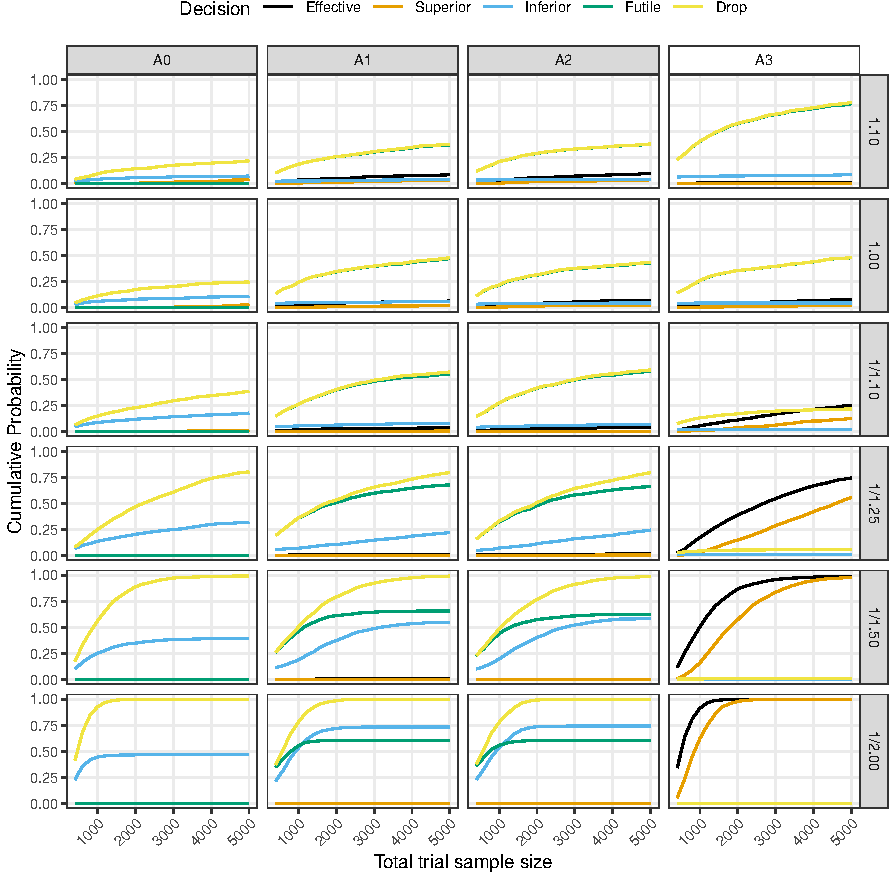
\includegraphics{ASCOT_simulations_5_files/figure-latex/unnamed-chunk-2-1.pdf}
\caption{\label{fig:unnamed-chunk-2}Probability of decision for domain A treatments as trial progresses (white facets are the affected treatments).}
\end{figure}

\begin{figure}
\centering
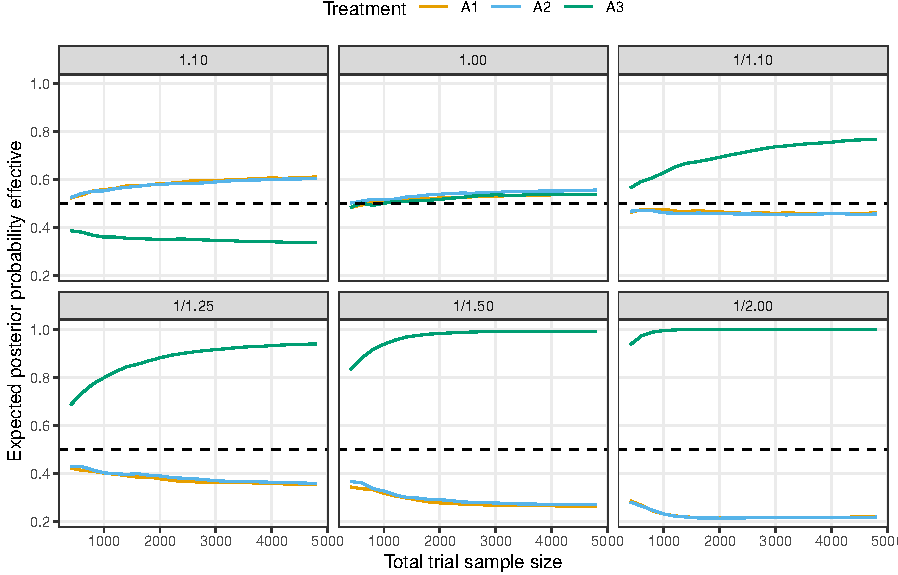
\includegraphics{ASCOT_simulations_5_files/figure-latex/unnamed-chunk-3-1.pdf}
\caption{\label{fig:unnamed-chunk-3}Expected posterior probability treatment in domain A is effective as trial progresses.}
\end{figure}

\begin{figure}
\centering
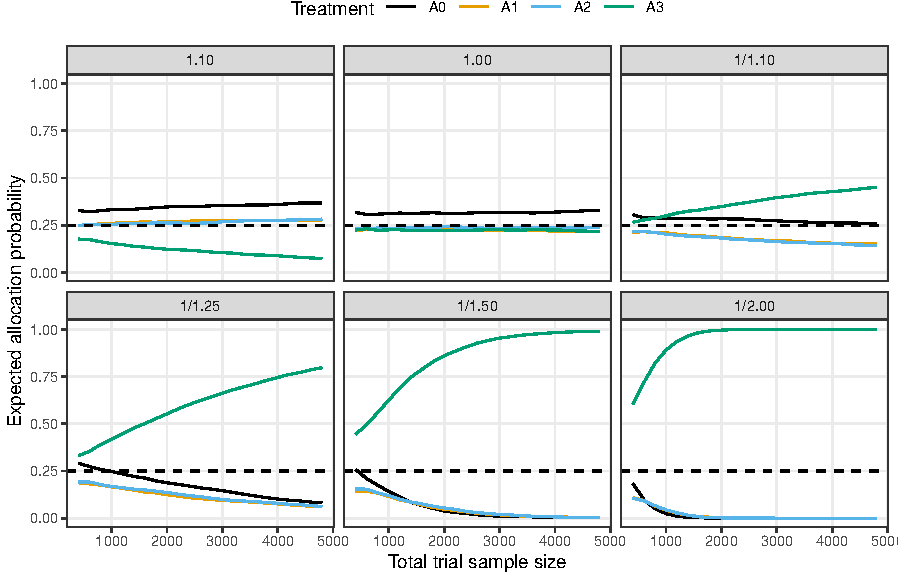
\includegraphics{ASCOT_simulations_5_files/figure-latex/fig6-1.pdf}
\caption{\label{fig:fig6}Expected allocation probability in domain A treatments as trial progresses. Affected treatments are \(A_3\).}
\end{figure}

\begin{figure}
\centering
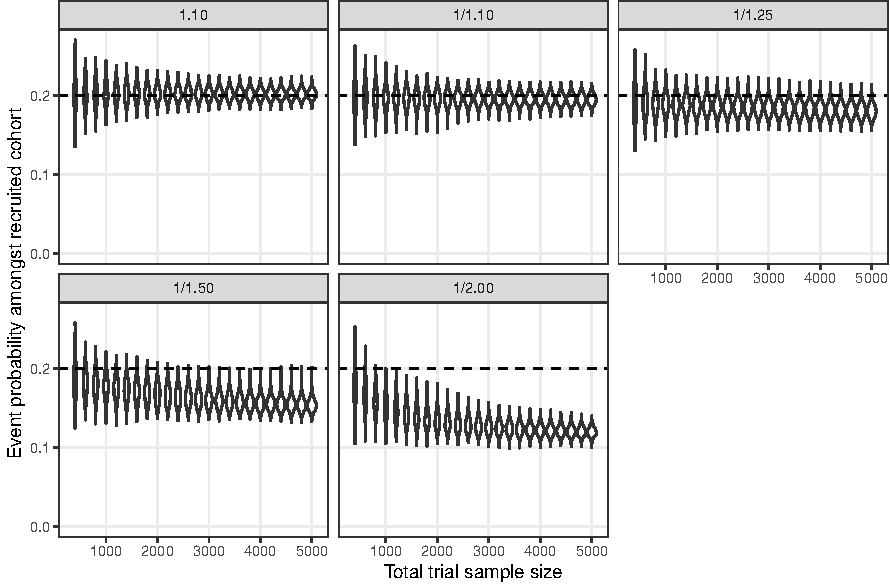
\includegraphics{ASCOT_simulations_5_files/figure-latex/fig7-1.pdf}
\caption{\label{fig:fig7}Probability of response as trial progresses.}
\end{figure}

\begin{figure}
\centering
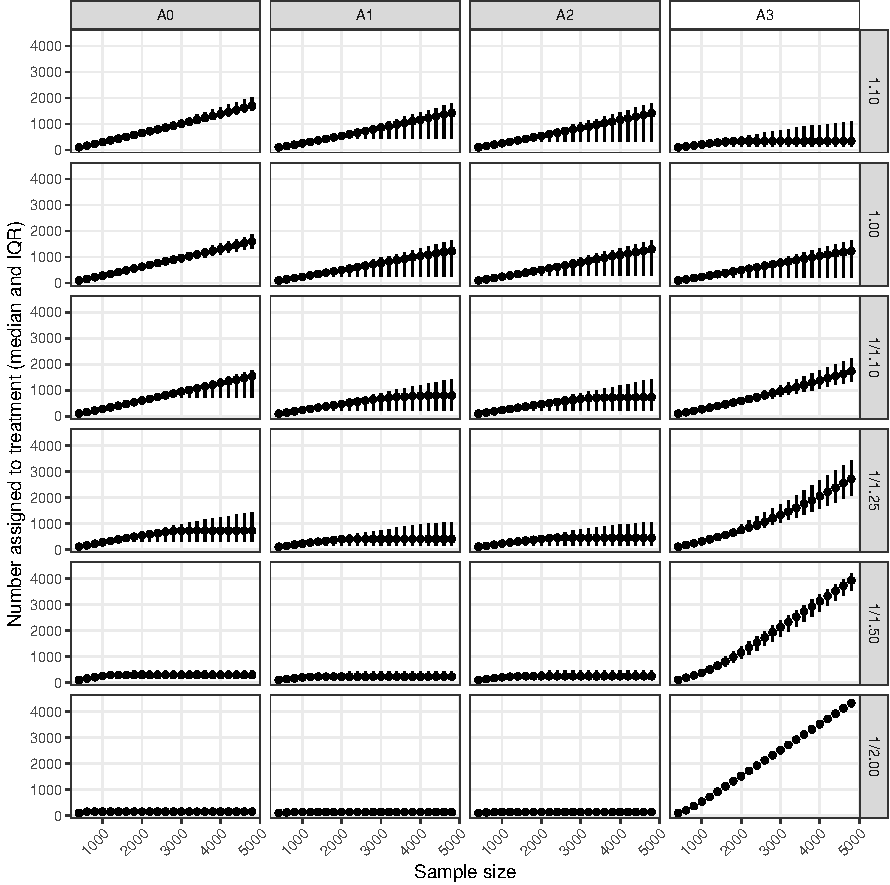
\includegraphics{ASCOT_simulations_5_files/figure-latex/unnamed-chunk-5-1.pdf}
\caption{\label{fig:unnamed-chunk-5}Number assigned to each treatment.}
\end{figure}

\begin{figure}
\centering
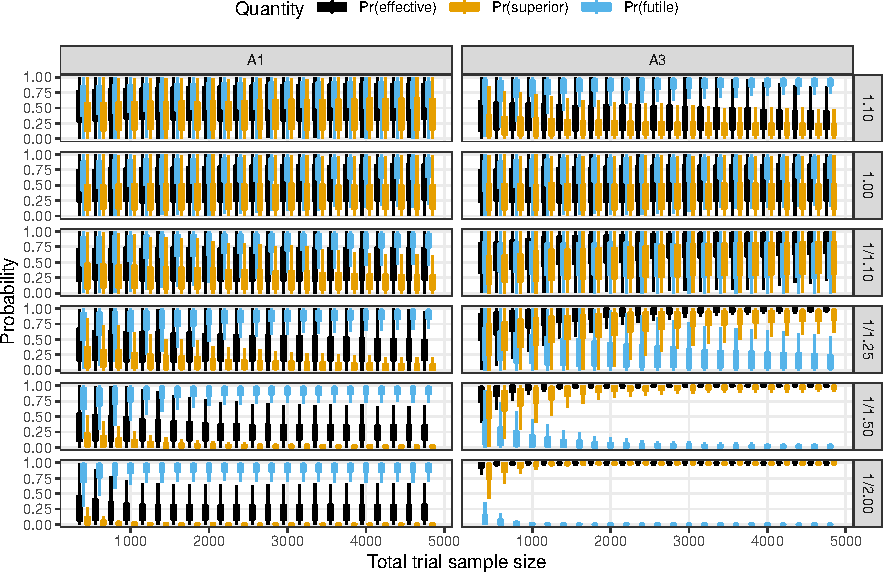
\includegraphics{ASCOT_simulations_5_files/figure-latex/unnamed-chunk-7-1.pdf}
\caption{\label{fig:unnamed-chunk-7}Distribution of treatment quantities.}
\end{figure}

\clearpage

\hypertarget{domain-b-3-treatments-one-as-standard-of-care}{%
\subsection{Domain B (3 treatments, one as standard of care)}\label{domain-b-3-treatments-one-as-standard-of-care}}

\hypertarget{one-treatment-effect-1}{%
\subsubsection{One Treatment Effect}\label{one-treatment-effect-1}}

\begin{figure}
\centering
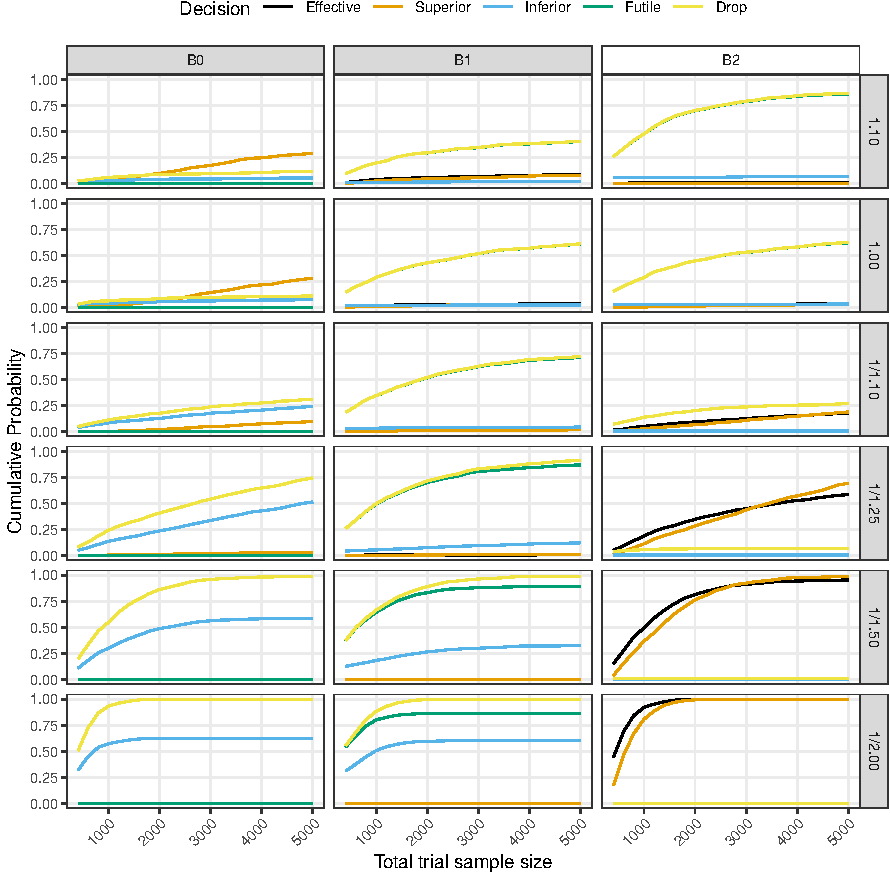
\includegraphics{ASCOT_simulations_5_files/figure-latex/unnamed-chunk-9-1.pdf}
\caption{\label{fig:unnamed-chunk-9}Probability of decision for domain B treatments as trial progresses (white facets are the affected treatments).}
\end{figure}

\begin{figure}
\centering
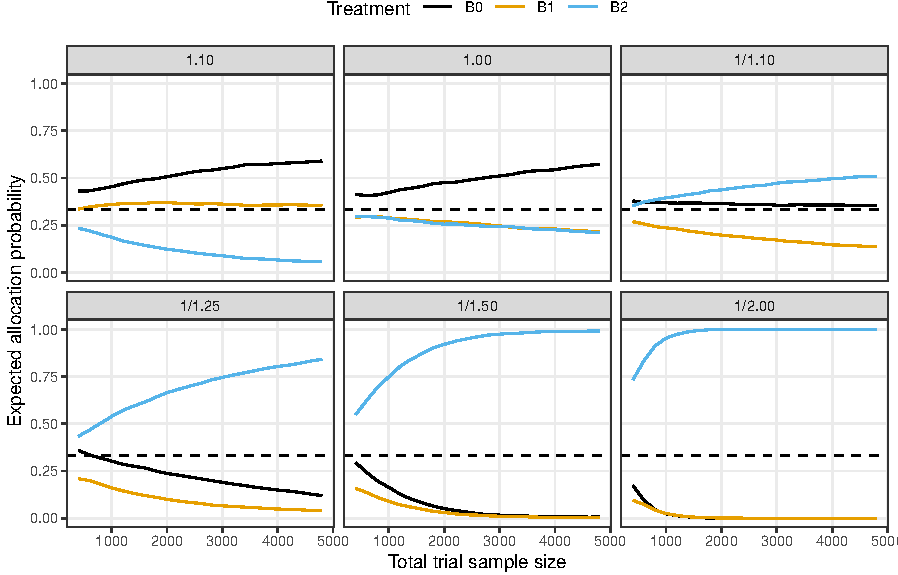
\includegraphics{ASCOT_simulations_5_files/figure-latex/unnamed-chunk-10-1.pdf}
\caption{\label{fig:unnamed-chunk-10}Expected allocation probability in domain B treatments as trial progresses. Affected treatments are \(A_3\).}
\end{figure}

\clearpage

\hypertarget{domain-c-2-treatments-one-as-standard-of-care}{%
\subsection{Domain C (2 treatments, one as standard of care)}\label{domain-c-2-treatments-one-as-standard-of-care}}

\hypertarget{one-treatment-effect-2}{%
\subsubsection{One Treatment Effect}\label{one-treatment-effect-2}}

\begin{figure}
\centering
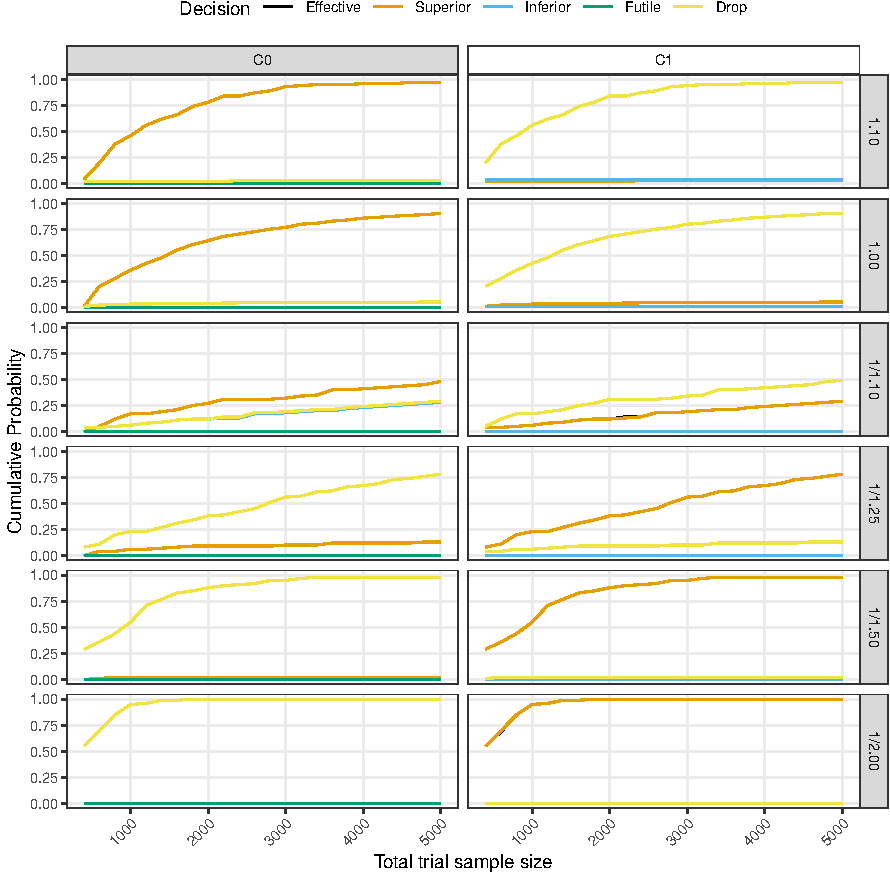
\includegraphics{ASCOT_simulations_5_files/figure-latex/unnamed-chunk-12-1.pdf}
\caption{\label{fig:unnamed-chunk-12}Probability of decision for domain C treatments as trial progresses (white facets are the affected treatments).}
\end{figure}

\begin{figure}
\centering
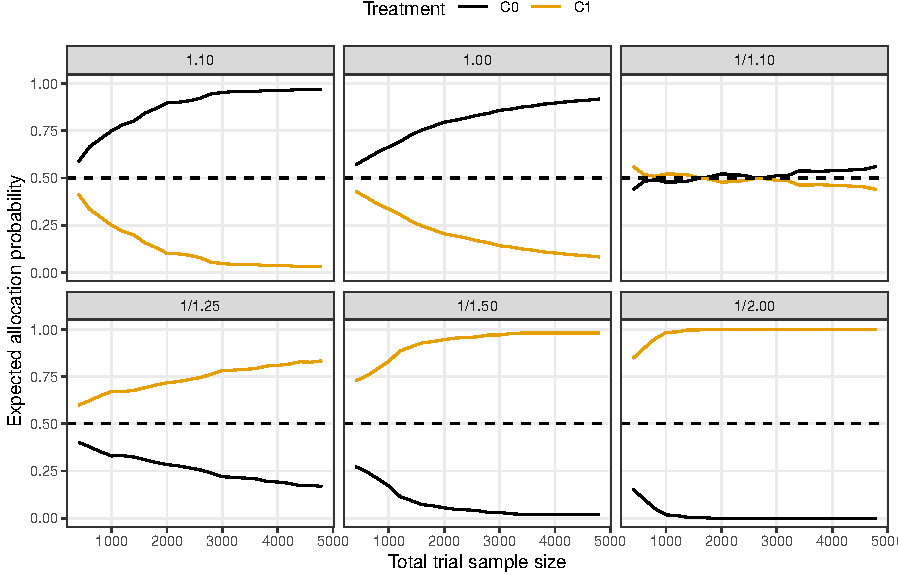
\includegraphics{ASCOT_simulations_5_files/figure-latex/unnamed-chunk-13-1.pdf}
\caption{\label{fig:unnamed-chunk-13}Expected allocation probability in domain C treatments as trial progresses. Affected treatments are \(A_3\).}
\end{figure}

\end{document}
